\chapter{Kendali Hormon atas Perkembangbiakan}\label{ch:b2:reproductive-hormones}

Tiap bulan, menurut jadwal yang tepat dalam selang satu atau dua hari
selama tiga puluh tahun, satu \omterm{def:b2:mammal-reproduction:ovary}{folikel} matang, satu sel telur
dilepaskan, pelapis rahimnya dibangun lalu, kecuali kalau sebuah
lembaga telah tiba, dirobohkan. Tidak ada jam di dalam tubuhnya yang
berdetak pada laju ini; iramanya muncul dari sebuah percakapan antara
tiga organ --- hipotalamus, hipofisis, dan ovarium --- yang di dalamnya
tiap hormonnya mengendalikan pelepasan hormon berikutnya dan yang
terakhir mengendalikan yang pertama. Bab ini membongkar percakapan itu:
sumbu yang menjalankan kedua kelaminnya, kendali tonik atas testisnya,
kendali berdaur atas ovariumnya beserta peralihannya yang luar biasa
dari umpan balik negatif ke positif, serta cara sumbunya dilangkahi
oleh kehamilan, oleh obat, dan oleh klinik.

\section{Sumbunya}

\begin{definition}[Sumbu hipotalamus-hipofisis-gonad]\label{def:b2:reproductive-hormones:axis}
\index{hormon pelepas gonadotropin}\index{hormon lutein}%
\index{hormon perangsang folikel}\index{umpan balik negatif!hormon}
Neuron \emph{hipotalamus} menyekresikan \emph{GnRH}
(hormon pelepas gonadotropin, sebuah peptida berisi sepuluh asam amino)
ke dalam pembuluh porta kecil yang menuju \emph{hipofisis anterior},
dalam \emph{denyut} pendek tiap satu sampai dua jam. GnRH membuat
hipofisisnya menyekresikan dua hormon glikoprotein ke dalam peredaran
umum, yaitu \emph{gonadotropin} \emph{LH} (hormon lutein) dan
\emph{FSH} (hormon perangsang \omterm{def:b2:mammal-reproduction:ovary}{folikel}). Keduanya bekerja pada
\emph{gonadnya}: LH pada sel pembuat steroid (\omterm{def:b2:mammal-reproduction:testis}{sel Leydig},
sel teka, dan sel lutein), FSH pada sel yang mengasuh gametnya
(\omterm{def:b2:mammal-reproduction:testis}{sel Sertoli} dan sel granulosa). Gonadnya menjawab dengan steroid ---
\emph{testosteron}, \emph{estradiol}, \emph{progesteron} --- dan
dengan peptida \emph{inhibin}, dan semuanya mengumpanbalik kepada
hipotalamus dan hipofisisnya: steroidnya kepada keduanya, kebanyakan
secara \emph{negatif}; inhibinnya kepada FSH saja. Hasilnya adalah
sebuah gelung teratur yang di dalamnya keluaran gonadnya ditahan pada
sebuah titik acuan, dan rancangan tiga tingkat yang sama menjalankan
kelenjar tiroid serta korteks adrenalnya. Mekanisme yang lewatnya
hormon ini bekerja pada selnya adalah pokok
\cref{ch:b2:cell-signalling}.
\end{definition}

\begin{omfigure}
\begin{tikzpicture}[every node/.style={font=\scriptsize}, >=stealth]
  \node[draw, rounded corners, fill=omDef!15, align=center, minimum width=3cm] (hyp) at (0,4.2) {hipotalamus\\GnRH, dalam denyut};
  \node[draw, rounded corners, fill=omDef!15, align=center, minimum width=3cm] (pit) at (0,2.2) {hipofisis anterior\\LH dan FSH};
  \node[draw, rounded corners, fill=omProp!20, align=center, minimum width=3cm] (gon) at (0,0) {gonad\\steroid, inhibin};
  \node[draw, rounded corners, fill=omExo!25, align=center, minimum width=3cm] (tar) at (5.2,0) {jaringan sasaran\\gametogenesis, saluran,\\ciri kelamin sekunder};
  \draw[->, thick] (hyp) -- (pit) node[midway, right] {pembuluh porta};
  \draw[->, thick] (pit) -- (gon) node[midway, right] {darah};
  \draw[->, thick] (gon) -- (tar);
  \draw[->, thick, omThm] (gon.west) .. controls (-3.0,0) and (-3.0,2.2) .. (pit.west);
  \draw[->, thick, omThm] (gon.west) .. controls (-4.6,0) and (-4.6,4.2) .. (hyp.west);
  \node[omThm, anchor=east, align=right] at (-3.9,1.2) {ke hipofisisnya:\\steroid $(-)$,\\inhibin $(-)$ pada FSH};
  \node[omThm, anchor=east, align=right] at (-3.9,3.6) {ke hipotalamusnya:\\steroid $(-)$\\(estradiol $(+)$\\pada pertengahan daurnya)};
\end{tikzpicture}

{\small Sumbunya: GnRH hipotalamus menggerakkan LH dan FSH hipofisis,
yang menggerakkan gonadnya; steroid dan inhibin gonadnya mengumpanbalik
secara negatif kepada kedua tingkat atasnya --- kecuali umpan balik
positif estradiol yang singkat, yang memicu \omterm{def:b2:mammal-reproduction:ovary}{ovulasi}.}
\end{omfigure}

\begin{proposition}[Mengapa denyutnya berarti]\label{prop:b2:reproductive-hormones:pulses}
\index{sekresi berdenyut}\index{penyahpekaan reseptor}
Hipofisisnya menanggapi GnRH hanya kalau GnRH-nya tiba dalam denyut.
Sebuah sel yang terpapar sebuah hormon secara sinambung membuang
reseptor hormonnya dari permukaannya (\emph{penyahpekaan}); kalau
lumbung reseptornya diisi kembali pada laju $s$, dibuang pada laju
basal $d$ dan, dengan hadirnya hormon $H$, pada laju tambahan $iH$,
maka
\[
\frac{\mathrm{d}R}{\mathrm{d}t} = s - (d + iH)\,R, \qquad R^* = \frac{s}{d + iH},
\]
sehingga $H$ tinggi yang sinambung mendorong cacah reseptornya ke
keadaan tunak yang rendah lalu selnya membisu, sedangkan denyut pendek
yang terpisah oleh selang tanpa hormon membiarkan lumbungnya pulih
(tetapan waktunya $1/d$) di antaranya. Sebuah denyut GnRH tiap sembilan
puluh menit menjaga hipofisisnya tetap menanggap; sebuah infus tetap,
atau agonis GnRH yang bekerja lama, mematikannya dalam beberapa hari
--- itulah dasar obat yang menekan sumbunya pada kanker prostat,
endometriosis, dan pubertas dini. Frekuensi denyutnya juga menyandikan
keterangan: denyut yang cepat memihak LH, denyut yang lambat memihak
FSH.
\end{proposition}
\begin{proof}[Bukti eksperimental]
Knobil (1978--1980) merusak neuron GnRH kera resus, yang meniadakan LH,
FSH, dan daurnya, lalu menggantikan GnRH-nya lewat pompa: satu denyut
tiap jam memulihkan gonadotropin dan daur \omterm{def:b2:mammal-reproduction:ovary}{ovulasi} yang normal; takaran
harian yang sama yang diberikan secara sinambung memulihkannya selama
beberapa hari lalu LH dan FSH-nya runtuh ke nol; kembali kepada
denyutnya memulihkannya lagi. Pola pengantarannya, bukan jumlahnya,
itulah isyaratnya.
\end{proof}

\begin{omfigure}
\begin{tikzpicture}
\begin{axis}[
  width=0.8\linewidth, height=5.4cm,
  axis x line=bottom, axis y line=left,
  xmin=0, xmax=40, ymin=0, ymax=1.2,
  xlabel={hari}, ylabel={LH plasma (relatif)},
  xlabel style={font=\small, at={(axis description cs:0.5,-0.13)}, anchor=north},
  ylabel style={font=\small},
  tick label style={font=\small}, xtick={0,10,20,30,40}, ytick={0,0.5,1},
  clip=false,
]
\addplot[very thick, omDef, domain=0:10, samples=2] {1};
\addplot[very thick, omThm, domain=10:25, samples=60] {exp(-(x-10)/3)};
\addplot[very thick, omDef, domain=25:40, samples=60] {1-exp(-(x-25)/2)};
\fill[omDef!15] (axis cs:0,1.05) rectangle (axis cs:10,1.15); \node[font=\scriptsize] at (axis cs:5,1.1) {denyut tiap jam};
\fill[omThm!15] (axis cs:10,1.05) rectangle (axis cs:25,1.15); \node[font=\scriptsize] at (axis cs:17.5,1.1) {infus sinambung};
\fill[omDef!15] (axis cs:25,1.05) rectangle (axis cs:40,1.15); \node[font=\scriptsize] at (axis cs:32.5,1.1) {denyut lagi};
\end{axis}
\end{tikzpicture}

{\small Percobaan Knobil, secara skematik. Pada seekor kera yang neuron
GnRH-nya sendiri telah dirusak, denyut GnRH tiap jam mempertahankan
LH-nya; beralih ke infus sinambung dengan jumlah harian yang sama
memadamkannya dalam beberapa hari, dan denyutnya memulihkannya.}
\end{omfigure}

\begin{omfigure}
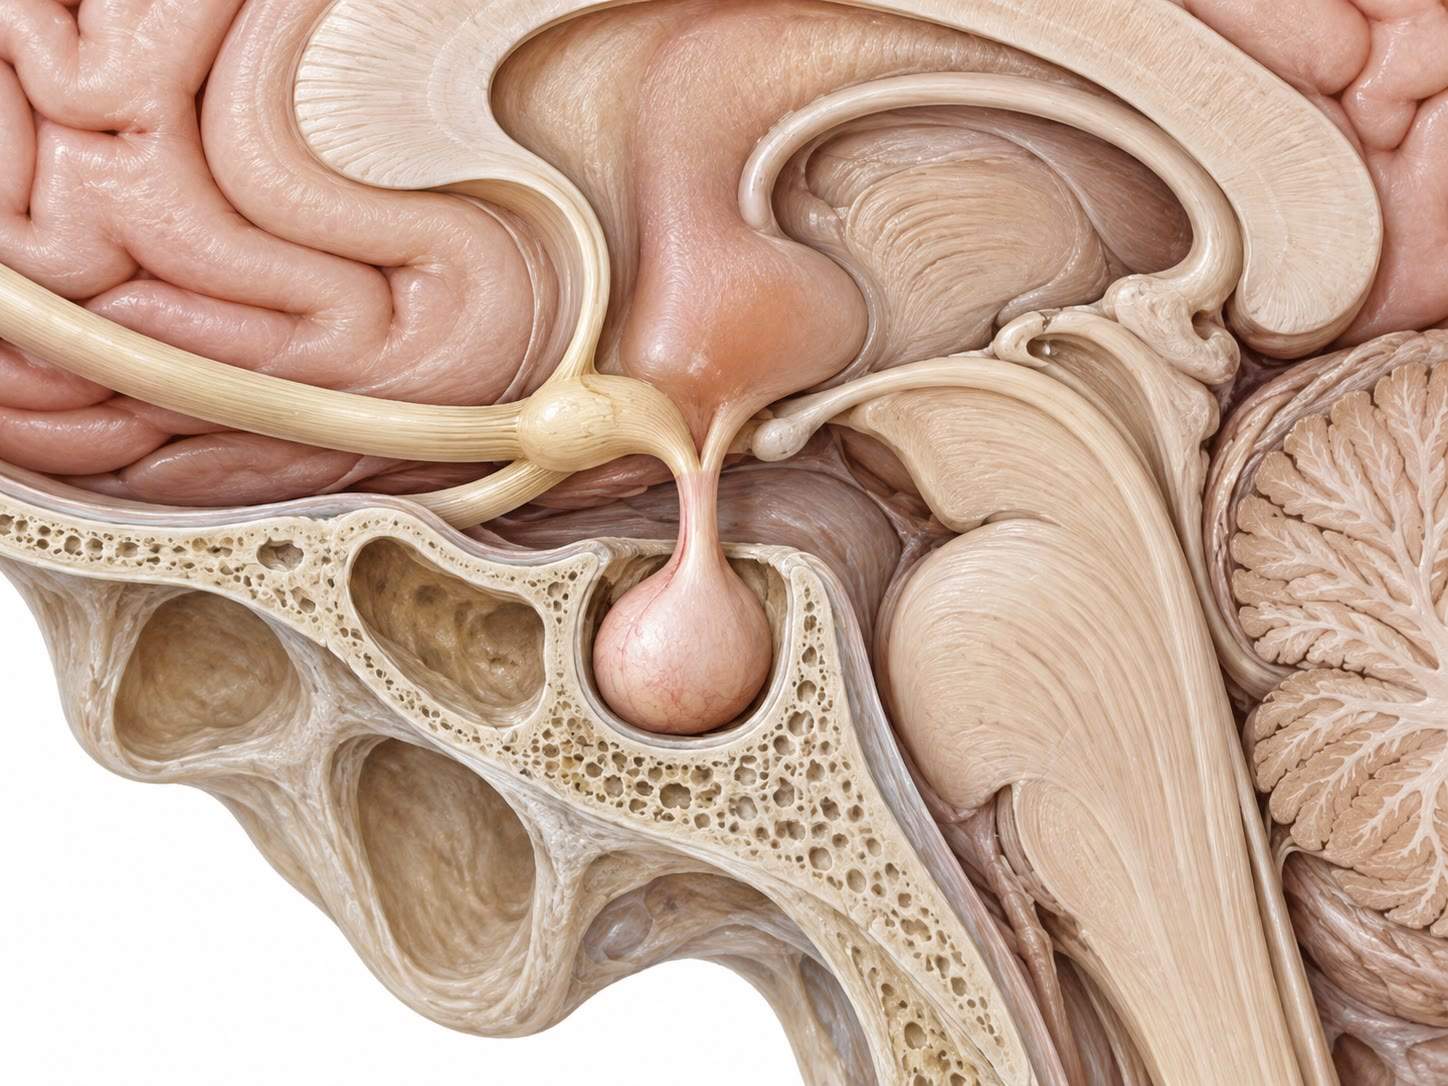
\includegraphics[width=0.55\linewidth]{images/book4/ai/b4-09-hypothalamus-pituitary.jpg}

{\small Dasar otaknya dalam potongan sagital: hipotalamusnya di atas,
tangkainya, dan hipofisisnya di dalam kantung tulangnya --- perangkat
keras sumbunya.}
\end{omfigure}

\section{Yang jantan: kendali tonik}

\begin{proposition}[Kendali atas testis]\label{prop:b2:reproductive-hormones:testis}
\index{testosteron}\index{inhibin}
LH bekerja pada \omterm{def:b2:mammal-reproduction:testis}{sel Leydig}, yang membuat \emph{testosteron}
(\qtyrange{3}{10}{ng/mL} di dalam darah seorang pria dewasa, seratus
kali lebih banyak di dalam testisnya). FSH bekerja pada \omterm{def:b2:mammal-reproduction:testis}{sel Sertoli},
yang --- bersama testosteron setempat --- menyokong \omterm{def:b2:mammal-reproduction:testis}{spermatogenesis}
dan menyekresikan \emph{inhibin}. Testosteronnya mengumpanbalik kepada
hipotalamus dan hipofisisnya untuk menahan LH tetap rendah; inhibinnya
mengumpanbalik kepada hipofisisnya untuk menahan FSH tetap rendah.
Kedua gelungnya \emph{negatif} dan sistemnya bersifat \emph{tonik}:
kadar hormonnya berayun mengikuti denyutnya dan mengikuti harinya
(tertinggi pada pagi hari) tetapi tidak berdaur, dan spermanya dibuat
sinambung. Testosteronnya juga membangun serta memelihara kelenjar dan
saluran tambahannya, janggutnya, suaranya, otot dan tulangnya,
penghasilan sel darah merahnya, dan gairahnya, serta pada janinnya
membuat tubuh jantannya (\cref{ch:b2:mammal-reproduction}). Pengebirian
membuangnya: LH dan FSH-nya naik beberapa kali lipat karena kehilangan
umpan baliknya, dan ciri sekundernya menyusut; testosteron yang
disuntikkan memulihkan cirinya --- tetapi tidak kesuburannya, karena ia
juga menekan LH dan dengan demikian menekan testosteron di dalam
testisnya yang dituntut \omterm{def:b2:mammal-reproduction:testis}{spermatogenesis}. Inilah sebabnya steroid
anabolik membuat pria mandul.
\end{proposition}
\begin{proof}[Bukti eksperimental]
Berthold (1849) mengebiri ayam jantan muda: jenggernya mengerut dan
mereka tidak berkokok maupun berkelahi. Sebuah testis yang dicangkokkan
ke dalam perut seekor ayam yang dikebiri, dan di situ ia menumbuhkan
pasokan darah baru tetapi tidak saraf, memulihkan jengger, kokok, dan
perkelahiannya: testisnya bekerja lewat darahnya --- peragaan pertama
sebuah sekresi dalam, lima puluh tahun sebelum kata hormon.
Testosteron diisolasi dan disintesis pada 1935.
\end{proof}

\section{Yang betina: sebuah daur dengan sakelar}

\begin{definition}[Daur ovarium dan daur rahim]\label{def:b2:reproductive-hormones:cycle}
\index{daur haid}\index{fase folikel}\index{fase lutein}%
\index{lonjakan LH}\index{endometrium}
Daurnya dihitung dari hari pertama haidnya dan berlangsung kira-kira 28
hari. \emph{Fase \omterm{def:b2:mammal-reproduction:ovary}{folikel}} (hari 1--14): FSH, yang terbebas dari umpan
balik oleh matinya \omterm{def:b2:mammal-reproduction:ovary}{korpus luteum} sebelumnya, merekrut sekelompok
\omterm{def:b2:mammal-reproduction:ovary}{folikel}; \omterm{def:b2:mammal-reproduction:ovary}{folikelnya} menyekresikan \emph{estradiol}, yang naik mantap;
estradiol dan inhibinnya menurunkan FSH, dan hanya \omterm{def:b2:mammal-reproduction:ovary}{folikel} dengan
reseptor FSH terbanyak yang selamat dari penurunannya --- yaitu folikel
dominannya. Di dalam rahimnya, estradiolnya membangun kembali
\emph{endometrium} (fase proliferasi) lalu mengencerkan lendir
serviksnya. \emph{\omterm{def:b2:mammal-reproduction:ovary}{Ovulasi}} (hari ke-14): ketika estradiolnya telah
tinggal di atas kira-kira \qty{200}{pg/mL} selama satu setengah hari,
umpan baliknya pada hipotalamus dan hipofisisnya beralih dari negatif
menjadi \emph{positif}; LH-nya naik sepuluh kali lipat dalam sehari ---
itulah \emph{lonjakan LH} --- dan kira-kira 36 jam sesudah awalnya
\omterm{def:b2:mammal-reproduction:ovary}{folikelnya} pecah lalu melepaskan oositnya. \emph{Fase lutein} (hari
15--28): \omterm{def:b2:mammal-reproduction:ovary}{folikel} yang telah kosong menjadi \omterm{def:b2:mammal-reproduction:ovary}{korpus luteum}, yang di bawah
LH menyekresikan \emph{progesteron} (\qtyrange{10}{20}{ng/mL}) dan
estradiol; progesteronnya menjadikan endometriumnya menyekresi,
mengentalkan lendirnya, menaikkan suhu tubuh basalnya
\qty{0.3}{\celsius}, dan bersama estradiolnya menekan LH serta FSH.
\omterm{def:b2:mammal-reproduction:ovary}{Korpus luteumnya} berumur kira-kira 14 hari; kecuali kalau hCG dari
sebuah lembaga menyelamatkannya, ia menyusut, progesteron dan
estradiolnya turun, endometriumnya luruh (\emph{haid}), FSH-nya naik,
lalu daur berikutnya dimulai. Fase luteinnya tetap 14 hari; keragaman
panjang daurnya adalah keragaman fase \omterm{def:b2:mammal-reproduction:ovary}{folikelnya}.
\end{definition}

\begin{omfigure}
\begin{tikzpicture}
\begin{axis}[
  width=0.94\linewidth, height=6.4cm,
  axis x line=bottom, axis y line=left,
  xmin=0, xmax=28, ymin=0, ymax=1.15,
  xlabel={hari daurnya}, ylabel={hormon (relatif terhadap puncaknya)},
  xlabel style={font=\small, at={(axis description cs:0.5,-0.11)}, anchor=north},
  ylabel style={font=\small},
  tick label style={font=\small}, xtick={0,7,14,21,28}, ytick={0,0.5,1},
  legend style={font=\scriptsize, at={(0.5,-0.25)}, anchor=north, draw=none, legend columns=4},
  clip=false,
]
\addplot[very thick, omThm, domain=0:28, samples=120] {0.1 + 0.9*exp(-((x-14)^2)/0.9)};
\addlegendentry{LH}
\addplot[very thick, omProp, domain=0:28, samples=120] {0.35*exp(-x/6) + 0.15 + 0.35*exp(-((x-14)^2)/1.2)};
\addlegendentry{FSH}
\addplot[very thick, omDef, domain=0:28, samples=160] {0.1 + 0.9*exp(-((x-12.5)^2)/6) + 0.4*exp(-((x-21)^2)/12)};
\addlegendentry{estradiol}
\addplot[very thick, omExo!70!black, domain=0:28, samples=160] {0.03 + 0.97*exp(-((x-21)^2)/12)*(x>14)};
\addlegendentry{progesteron}
\draw[dashed, gray] (axis cs:14.5,0) -- (axis cs:14.5,1.1); \node[font=\scriptsize, anchor=south] at (axis cs:14.5,1.1) {ovulasi};
\node[font=\scriptsize, anchor=north] at (axis cs:7,1.1) {fase folikel};
\node[font=\scriptsize, anchor=north] at (axis cs:21.5,1.1) {fase lutein};
\end{axis}
\end{tikzpicture}

{\small Hormon daurnya. Estradiol dari \omterm{def:b2:mammal-reproduction:ovary}{folikel} yang tumbuh naik
sepanjang \omterm{def:b2:reproductive-hormones:cycle}{fase folikelnya} dan, melewati sebuah ambang, memicu
\omterm{def:b2:reproductive-hormones:cycle}{lonjakan LH}; \omterm{def:b2:mammal-reproduction:ovary}{ovulasi} menyusul kira-kira 36 jam kemudian; \omterm{def:b2:mammal-reproduction:ovary}{korpus
luteumnya} lalu menyekresikan progesteron selama dua pekan lalu mati.}
\end{omfigure}

\begin{omfigure}
\begin{tikzpicture}[every node/.style={font=\scriptsize}]
  % endometrium thickness over the cycle
  \draw[thick, ->] (0,0) -- (12.4,0) node[right] {hari};
  \foreach \x/\l in {0/1, 2.1/5, 6.0/14, 12/28} \draw (\x,0.08) -- (\x,-0.08) node[below] {\l};
  \fill[omThm!25] (0,0) -- (0,1.4) .. controls (0.8,1.2) and (1.6,0.5) .. (2.1,0.35) -- (2.1,0) -- cycle;
  \fill[omDef!20] (2.1,0) -- (2.1,0.35) .. controls (3.5,0.6) and (5.2,1.3) .. (6.0,1.5) -- (6.0,0) -- cycle;
  \fill[omExo!35] (6.0,0) -- (6.0,1.5) .. controls (8,1.8) and (11,1.9) .. (12,1.6) -- (12,0) -- cycle;
  \node at (1.0,1.8) {haid};
  \node at (4.0,1.8) {proliferasi (estradiol)};
  \node at (9,2.2) {sekresi (progesteron): kelenjar, glikogen, arteri spiral};
  \node[anchor=east] at (-0.1,0.8) {endometrium};
\end{tikzpicture}

{\small Daur rahimnya. \omterm{def:b2:reproductive-hormones:cycle}{Endometriumnya} luruh saat haid, dibangun
kembali di bawah estradiol, lalu dijadikan menyekresi di bawah
progesteron, siap menerima sebuah \omterm{def:b2:mammal-reproduction:implantation}{blastosista} sekitar hari ke-21;
ketika progesteronnya turun, ia luruh lagi.}
\end{omfigure}

\begin{omfigure}
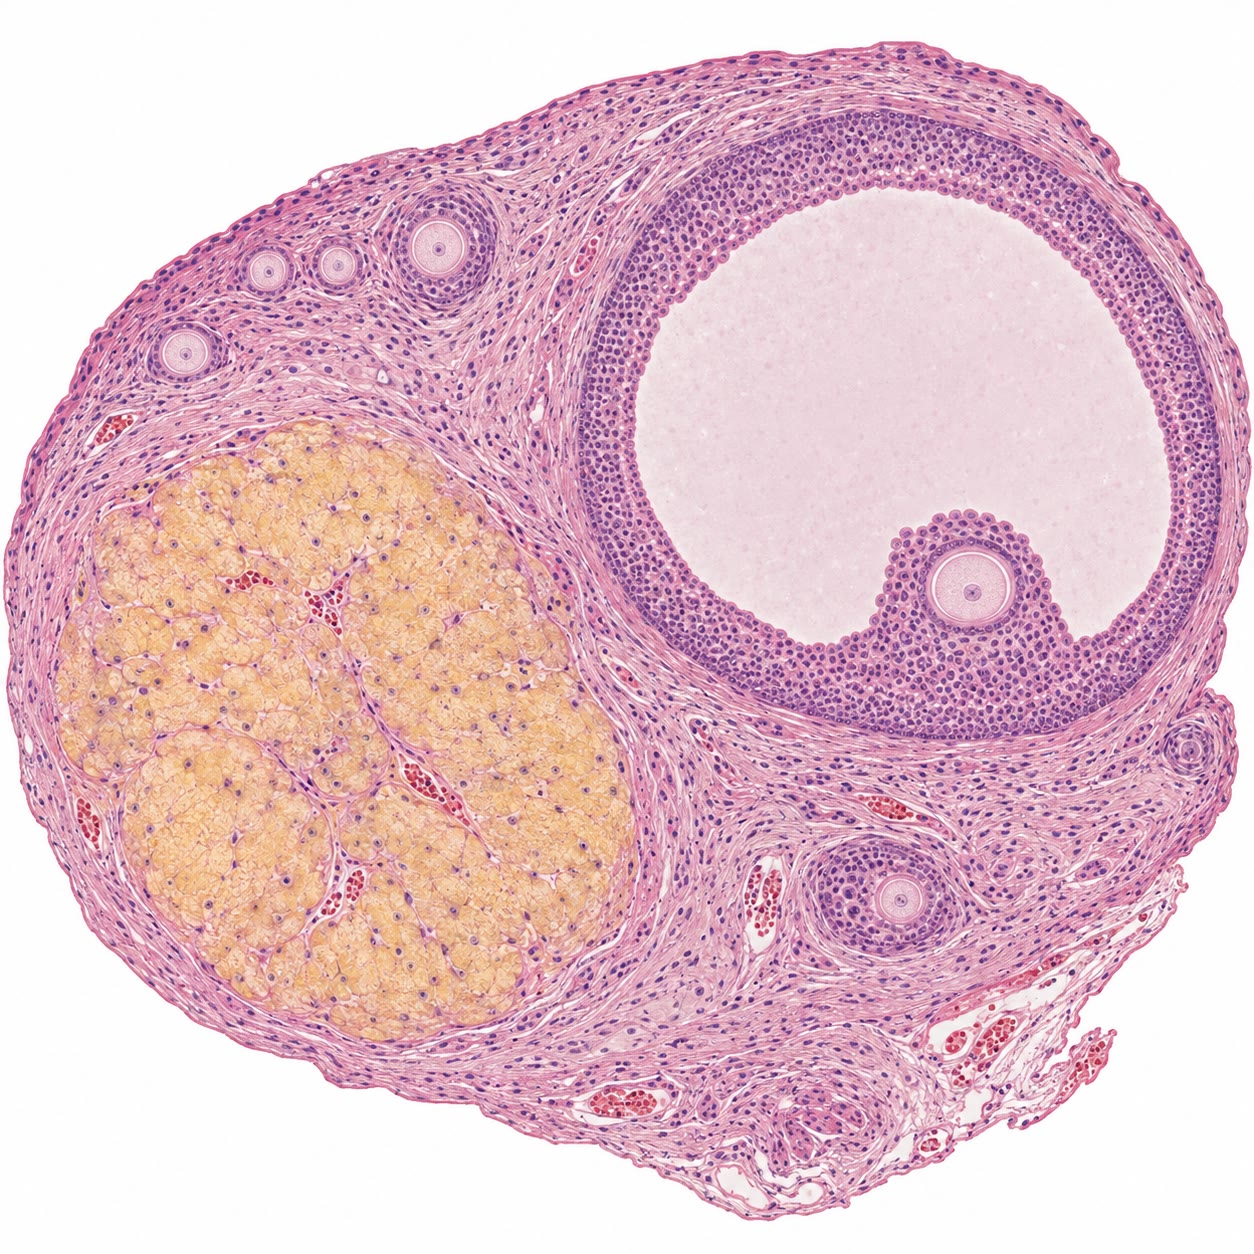
\includegraphics[width=0.46\linewidth]{images/book4/ai/b4-09-ovary-histology.jpg}

{\small Sebuah ovarium dalam potongan: sebuah \omterm{def:b2:mammal-reproduction:ovary}{folikel} matang dengan
rongga dan oositnya, \omterm{def:b2:mammal-reproduction:ovary}{folikel} primordial kecil di bawah permukaannya,
dan sebuah \omterm{def:b2:mammal-reproduction:ovary}{korpus luteum} dari daur sebelumnya.}
\end{omfigure}

\begin{theorem}[Peralihan dari umpan balik negatif ke positif]\label{thm:b2:reproductive-hormones:switch}
\index{umpan balik positif!lonjakan LH}
Estradiol pada kadar rendah awal \omterm{def:b2:reproductive-hormones:cycle}{fase folikelnya}
menghambat LH dan FSH; estradiol di atas kira-kira \qty{200}{pg/mL},
yang bertahan lebih dari kira-kira \qty{36}{h}, melakukan kebalikannya:
ia membuat hipotalamusnya melepaskan ledakan GnRH dan hipofisisnya
menanggapinya dengan kenaikan LH sepuluh kali lipat. Mekanismenya
adalah perubahan tanda, bukan perubahan besaran: takaran tinggi yang
bertahan mengimbas di dalam hipofisisnya sebuah lumbung LH yang besar
dan kepekaan yang meninggi terhadap GnRH, dan di dalam hipotalamusnya
(lewat neuron kisspeptin) sebuah peralihan pembangkit denyut GnRH-nya
ke ragam lonjakan. Sakelarnya mengubah sebuah isyarat berjenjang ---
seberapa banyak estradiol yang dibuat \omterm{def:b2:mammal-reproduction:ovary}{folikelnya} --- menjadi sebuah
peristiwa serba-atau-tidak yang tepat harinya, dan itulah yang dituntut
\omterm{def:b2:mammal-reproduction:ovary}{ovulasi}; dan karena hanya \omterm{def:b2:mammal-reproduction:ovary}{folikel} yang besar dan matang yang sanggup
mempertahankan \qty{200}{pg/mL}, lonjakannya hanya menyala kalau ada
sebutir sel telur yang siap dilepaskan. Begitu \omterm{def:b2:mammal-reproduction:ovary}{ovulasinya} terjadi,
progesteron \omterm{def:b2:mammal-reproduction:ovary}{korpus luteumnya} memulihkan umpan balik negatifnya dan
tidak ada lonjakan kedua yang menyusul.
\end{theorem}
\begin{proof}[Bukti eksperimental]
Pada perempuan dan kera yang sumbunya ditekan, sebuah infus estradiol
yang menaikkan kadar plasmanya di atas \qty{200}{pg/mL} selama dua hari
diikuti sebuah \omterm{def:b2:reproductive-hormones:cycle}{lonjakan LH}; jumlah yang sama yang diberikan selama satu
hari, atau kadar yang lebih rendah selama tiga hari, tidak diikuti
lonjakan. Progesteron yang diberikan sebelum infusnya menghadang
lonjakannya; yang diberikan bersamaan memajukan dan memperkuatnya.
Ambang takaran dan lamanya itu menirukan waktu lonjakan alaminya dari
kenaikan estradiol alaminya.
\end{proof}

\section{Melangkahi daurnya}

\begin{proposition}[Kehamilan, laktasi, menopause]\label{prop:b2:reproductive-hormones:overrides}
\index{gonadotropin korion manusia}\index{menopause}
Sebuah lembaga yang berimplantasi menyekresikan \emph{hCG}, sebuah
hormon mirip LH yang mengikat reseptor LH lalu menjaga \omterm{def:b2:mammal-reproduction:ovary}{korpus luteumnya}
tetap hidup dan menyekresi melewati keempat belas harinya; pada pekan
kesepuluh, \omterm{def:b2:mammal-reproduction:placenta}{plasentanya} sendiri membuat cukup progesteron dan estrogen
untuk mempertahankan kehamilannya dan \omterm{def:b2:mammal-reproduction:ovary}{korpus luteumnya} dapat
dikesampingkan. Sepanjang kehamilannya, steroidnya yang tinggi menahan
LH dan FSH pada nol: tidak ada \omterm{def:b2:mammal-reproduction:ovary}{folikel} yang tumbuh dan tidak ada
\omterm{def:b2:mammal-reproduction:ovary}{ovulasi} yang terjadi. Sesudah kelahirannya, mengisap menaikkan
prolaktin lalu memperlambat denyut GnRH-nya, dan \omterm{def:b2:mammal-reproduction:ovary}{ovulasinya} tetap
tertekan berbulan-bulan. Pada \emph{menopause}, persediaan \omterm{def:b2:mammal-reproduction:ovary}{folikelnya}
habis: estradiol dan inhibinnya turun, dan, tanpa apa pun yang
mengumpanbalik, LH dan FSH-nya naik menjadi sepuluh kali kadarnya yang
dahulu lalu tetap di situ --- tanda sebuah kelenjar yang telah berhenti
menjawab.
\end{proposition}

\begin{proposition}[Kontrasepsi dan perkembangbiakan berbantuan]\label{prop:b2:reproductive-hormones:clinic}
\index{kontrasepsi!hormon}\index{pembuahan di luar tubuh}
Pil gabungan mengantarkan sebuah estrogen sintetis dan sebuah
progestin tiap hari: kadar steroidnya yang tetap menjaga FSH dan LH
tetap rendah, tidak ada \omterm{def:b2:mammal-reproduction:ovary}{folikel} yang direkrut, tidak ada kenaikan
estradiol yang terjadi, dan lonjakannya tidak pernah menyala;
progestinnya juga mengentalkan lendir serviksnya. Jeda tujuh harinya
membiarkan \omterm{def:b2:reproductive-hormones:cycle}{endometriumnya} berdarah; melewatkan pilnya lebih dari dua
hari berturut-turut membiarkan FSH-nya lolos dan sebuah \omterm{def:b2:mammal-reproduction:ovary}{folikel} dapat
tumbuh. Kontrasepsi darurat menunda lonjakannya beberapa hari dengan
takaran progestin yang besar. Pada \emph{\omterm{prop:b2:reproductive-hormones:clinic}{pembuahan di luar tubuh}},
sumbunya digerakkan ke arah sebaliknya: FSH harian selama sepuluh hari
melangkahi pemilihan satu folikel dominan lalu mematangkan sepuluh atau
lebih; sebuah antagonis GnRH mencegah lonjakan spontan yang terlalu
dini; sebuah suntikan hCG menggantikan lonjakannya, dan oositnya
dikumpulkan 34 sampai 36 jam kemudian, tepat sebelum mereka akan
dilepaskan; mereka dibuahi di dalam cawan lalu satu atau dua lembaganya
dipindahkan, sisanya dibekukan. Pada pria, testosteron dari luar atau
sebuah analog GnRH menekan \omterm{def:b2:mammal-reproduction:testis}{spermatogenesis} dengan menekan LH --- itulah
asas sebuah kontrasepsi hormon jantan, yang masih belum dipasarkan.
Semua ini adalah sumbu bagian pertama, yang dibaca terbalik.
\end{proposition}

\section{Latihan}

\begin{exercise}[$\star$]\label{exo:b2:reproductive-hormones:1}
Gambarkanlah sumbunya bagi yang jantan: ketiga tingkatnya, keempat
hormonnya, kedua gelung umpan baliknya, dan sel yang menjadi tempat
tiap hormonnya bekerja.
\end{exercise}

\begin{exercise}[$\star$]\label{exo:b2:reproductive-hormones:2}
Berikan fase daur ovarium dan daur rahimnya beserta harinya dan hormon
yang mendominasi masing-masingnya.
\end{exercise}

\begin{exercise}[$\star$]\label{exo:b2:reproductive-hormones:3}
Jelaskan bagaimana pil gabungan mencegah \omterm{def:b2:mammal-reproduction:ovary}{ovulasi}, dan mengapa
perdarahannya terjadi pada pekan tanpa pil.
\end{exercise}

\begin{exercise}[$\star$]\label{exo:b2:reproductive-hormones:4}
Apa yang terjadi pada LH, FSH, dan ciri kelamin sekunder seorang pria
dewasa yang dikebiri? Mana di antaranya yang dibalikkan testosteron
yang disuntikkan, dan mana yang tidak?
\end{exercise}

\begin{exercise}[$\star\star$]\label{exo:b2:reproductive-hormones:5}
Denyut GnRH datang tiap \qty{90}{min} pada \omterm{def:b2:reproductive-hormones:cycle}{fase folikelnya} dan
tiap \qty{4}{h} pada \omterm{def:b2:reproductive-hormones:cycle}{fase luteinnya}. Berapa denyut sehari pada
masing-masingnya? Hipofisisnya memihak LH pada denyut cepat dan FSH
pada denyut lambat: gonadotropin mana yang seharusnya naik lebih dahulu
ketika \omterm{def:b2:mammal-reproduction:ovary}{korpus luteumnya} mati, dan mengapa itu yang tepat?
\end{exercise}

\begin{exercise}[$\star\star$]\label{exo:b2:reproductive-hormones:6}
Ubahlah \qty{200}{pg/mL} estradiol (massa molar
\qty{272}{g/mol}) menjadi \unit{pmol/L}, dan \qty{15}{ng/mL}
progesteron (\qty{314}{g/mol}) menjadi \unit{nmol/L}. Berapa banyak
molekul estradiol yang ada di dalam satu mikroliter plasma pada ambang
lonjakannya?
\end{exercise}

\begin{exercise}[$\star\star$]\label{exo:b2:reproductive-hormones:7}
Daur seorang perempuan berlangsung 35 hari. Mengingat \omterm{def:b2:reproductive-hormones:cycle}{fase luteinnya}
tetap, pada hari keberapa ia berovulasi, dan hari mana yang subur kalau
spermanya bertahan tiga hari dan sel telurnya sehari? Mengapa cara
kalender gagal bagi daur yang tak teratur?
\end{exercise}

\begin{exercise}[$\star\star$]\label{exo:b2:reproductive-hormones:8}
Sebuah lembaga berimplantasi pada hari ke-21 sebuah daur 28 hari dan
hCG-nya, yang dimulai pada \qty{1}{IU/L}, berlipat dua tiap dua hari.
\omterm{def:b2:mammal-reproduction:ovary}{Korpus luteumnya} membutuhkan beberapa IU/L hCG pada hari ke-26 agar
bertahan. Apakah lembaganya tepat waktu? Apa yang akan terjadi kalau
\omterm{def:b2:mammal-reproduction:implantation}{implantasinya} tertunda sampai hari ke-25?
\end{exercise}

\begin{exercise}[$\star\star$]\label{exo:b2:reproductive-hormones:9}
Nyatakanlah apa yang ditunjukkan percobaan Knobil dan apa yang
disingkirkannya, lalu ramalkan pengaruh memberi seorang perempuan
agonis GnRH yang bekerja lama selama sebulan: pada LH-nya, pada
estradiolnya, pada \omterm{def:b2:reproductive-hormones:cycle}{endometriumnya}.
\end{exercise}

\begin{exercise}[$\star\star\star$]\label{exo:b2:reproductive-hormones:10}
Pada model reseptornya, ambillah $s = 100$ reseptor tiap jam, $d =
\qty{0.5}{h^{-1}}$ dan $iH = \qty{6}{h^{-1}}$ selagi hormonnya hadir.
Hitunglah cacah reseptor keadaan tunaknya tanpa hormon dan dengan
hormon sinambung. Dengan denyut dua menit tiap jam, hitunglah cacah
yang hilang tiap denyutnya dan bagian kekurangannya yang dipulihkan
sebelum denyut berikutnya, lalu simpulkan kadar tempat lumbungnya
menetap.
\end{exercise}

\begin{exercise}[$\star\star\star$]\label{exo:b2:reproductive-hormones:11}
Seorang perempuan pascamenopause memiliki LH dan FSH sepuluh kali kadar
seorang perempuan muda dan estradiol yang sangat rendah; seorang
perempuan dengan tumor hipofisis yang menyekresikan prolaktin memiliki
LH rendah, estradiol rendah, dan tanpa daur; seorang perempuan dengan
tumor sel granulosa memiliki estradiol tinggi, LH rendah, dan tanpa
daur. Jelaskan tiap tampangnya dari sumbunya.
\end{exercise}

\begin{exercise}[$\star\star\star$]\label{exo:b2:reproductive-hormones:12}
``Hormon yang sama menghambat lalu memicu \omterm{def:b2:reproductive-hormones:cycle}{lonjakan LH}.''
Jelaskan bagaimana estradiol dapat memiliki kedua pengaruh itu, mengapa
\omterm{def:b2:mammal-reproduction:ovary}{ovulasi} membutuhkan sebuah sakelar alih-alih sebuah tombol putar, dan
apa yang akan kacau dengan sebuah tombol putar.
\end{exercise}

\section{Soal: Sebuah Daur yang Diukur}

\begin{problem}[{Soal akhir pekan --- pengukuran hormon harian satu
daur dibaca untuk mendapatkan fasenya, hari ovulasinya, dan jendela
suburnya; ambang lonjakannya, jam korpus luteumnya, dan penyelamatan
hCG-nya dihitung; model reseptornya menjelaskan Knobil; dan sumbunya
digerakkan terbalik di dalam klinik, berakhir pada hari ovulasinya,
panjang fase luteinnya, jendela suburnya, dan ambang lonjakannya}]
\label{pb:b2:reproductive-hormones:1}
Darah dicuplik pada hari-hari terpilih sebuah daur seorang perempuan:

\begin{center}
\small
\begin{tabular}{lcccccccccc}
\hline
hari & 1 & 5 & 8 & 11 & 12 & 13 & 14 & 15 & 21 & 27 \\
\hline
estradiol (\unit{pg/mL}) & 40 & 60 & 110 & 210 & 260 & 310 & 220 & 150 & 160 & 50 \\
LH (\unit{IU/L}) & 5 & 5 & 6 & 7 & 8 & 20 & 65 & 15 & 4 & 4 \\
progesteron (\unit{ng/mL}) & 0.5 & 0.5 & 0.6 & 0.7 & 0.8 & 1.0 & 1.5 & 3 & 16 & 2 \\
suhu (\unit{\celsius}) & 36.4 & 36.4 & 36.4 & 36.4 & 36.4 & 36.4 & 36.4 & 36.5 & 36.8 & 36.7 \\
\hline
\end{tabular}
\end{center}

Haidnya mulai pada hari ke-1 dan mulai lagi pada hari ke-29.

\medskip
\noindent\textbf{Bagian I --- Membaca daurnya.}
\begin{enumerate}
  \item Kenalilah \omterm{def:b2:reproductive-hormones:cycle}{fase folikel} dan \omterm{def:b2:reproductive-hormones:cycle}{fase luteinnya} dari tabelnya,
        beserta hormon yang menandai masing-masingnya.
  \item Pada hari keberapa \omterm{def:b2:reproductive-hormones:cycle}{lonjakan LH-nya} memuncak? Kapan \omterm{def:b2:mammal-reproduction:ovary}{ovulasinya}
        terjadi?
  \item Berapa lama \omterm{def:b2:reproductive-hormones:cycle}{fase luteinnya}? Apakah ia sepadan dengan umur
        \omterm{def:b2:mammal-reproduction:ovary}{korpus luteumnya}?
  \item Jelaskan pergeseran suhunya dan mengapa ia menegaskan, tetapi
        tidak dapat meramalkan, \omterm{def:b2:mammal-reproduction:ovary}{ovulasinya}.
  \item Pada hari mana saja estradiolnya di atas \qty{200}{pg/mL}?
        Kaitkan lamanya dengan lonjakannya.
  \item Berikan jendela subur daur ini (sperma tiga hari, sel telur
        satu hari).
\end{enumerate}

\medskip
\noindent\textbf{Bagian II --- Angkanya.}
\begin{enumerate}[resume]
  \item Ubahlah estradiol hari ke-13 menjadi \unit{pmol/L}, dan
        progesteron hari ke-21 menjadi \unit{nmol/L}.
  \item Dengan faktor berapa LH naik dari hari ke-12 ke hari ke-14?
        Mengapa ia turun begitu cepat sesudahnya (waktu paruh LH
        kira-kira \qty{1}{h})?
  \item Kalau daur berikutnya perempuan ini memiliki \omterm{def:b2:reproductive-hormones:cycle}{fase folikel} 21
        hari, pada hari keberapa ia akan berovulasi dan berapa panjang
        daurnya?
  \item Sebuah lembaga berimplantasi 7 hari sesudah \omterm{def:b2:mammal-reproduction:ovary}{ovulasi}. Pada hari
        keberapa daur ini hCG-nya akan muncul, dan, dengan berlipat dua
        tiap dua hari dari \qty{1}{IU/L}, kadar berapa yang akan
        dicapainya pada hari ke-27?
  \item Jelaskan mengapa progesteron hari ke-27 sebesar \qty{2}{ng/mL}
        menunjukkan bahwa tidak ada lembaga yang berimplantasi.
  \item Berapa nilai progesteron dan estradiol hari ke-27 kalau ada
        yang berimplantasi?
\end{enumerate}

\medskip
\noindent\textbf{Bagian III --- Umpan balik dan denyutnya.}
\begin{enumerate}[resume]
  \item Jelaskan, dengan tanda umpan baliknya, mengapa FSH tertinggi
        pada awal daurnya dan mengapa biasanya hanya satu \omterm{def:b2:mammal-reproduction:ovary}{folikel} yang
        selamat.
  \item Pada model reseptornya dengan $s = 100$ tiap jam, $d =
        \qty{0.5}{h^{-1}}$, $iH = \qty{6}{h^{-1}}$, hitunglah $R^*$
        tanpa hormon dan di bawah hormon sinambung.
  \item Sebuah denyut berlangsung \qty{2}{min}. Dimulai dari $R^*$
        tanpa rangsangan, berapa reseptor yang dibuang satu denyutnya
        (pakailah hampiran linear $iHR\,\Delta t$)? Berapa bagian
        kekurangannya yang dipulihkan dalam satu jam sebelum denyut
        berikutnya (tetapan waktunya $1/d$), dan pada kadar berapa
        lumbungnya menetap?
  \item Pakailah angka ini untuk menjelaskan hasil Knobil.
  \item Seorang pria diberi agonis GnRH secara sinambung untuk kanker
        prostat. Ramalkanlah LH dan testosteronnya sesudah satu hari
        dan sesudah satu bulan, lalu jelaskan perbedaannya.
  \item Sel granulosa seorang perempuan gagal membuat inhibin.
        Ramalkanlah FSH dan LH-nya, serta akibatnya bagi perekrutan
        \omterm{def:b2:mammal-reproduction:ovary}{folikelnya}.
\end{enumerate}

\medskip
\noindent\textbf{Bagian IV --- Kliniknya.}
\begin{enumerate}[resume]
  \item Untuk \omterm{prop:b2:reproductive-hormones:clinic}{pembuahan di luar tubuh}, perempuan ini menerima FSH tiap
        hari sejak hari ke-2. Jelaskan mengapa sepuluh \omterm{def:b2:mammal-reproduction:ovary}{folikel} matang
        alih-alih satu.
  \item Mengapa sebuah antagonis GnRH ditambahkan sejak hari ke-6, dan
        apa yang akan terjadi tanpanya?
  \item hCG disuntikkan ketika \omterm{def:b2:mammal-reproduction:ovary}{folikelnya} masak; oositnya dikumpulkan
        35 jam kemudian. Berilah alasan bagi waktunya dari tabelnya.
  \item Sepuluh oosit dikumpulkan; \qty{70}{\%} terbuahi,
        \qty{40}{\%} lembaganya mencapai tahap \omterm{def:b2:mammal-reproduction:implantation}{blastosista}, dan tiap
        \omterm{def:b2:mammal-reproduction:implantation}{blastosista} yang dipindahkan berimplantasi dengan peluang
        $0.35$. Berapa harapan cacah \omterm{def:b2:mammal-reproduction:implantation}{blastosistanya}? Berapa peluang
        sedikitnya satu kehamilan kalau dua dipindahkan?
  \item Jelaskan mengapa pil gabungan, kalau diminum perempuan ini,
        akan menghasilkan sebuah tabel tanpa \omterm{def:b2:reproductive-hormones:cycle}{lonjakan LH} dan tanpa
        kenaikan progesteron.
  \item Sebuah kontrasepsi jantan berdasarkan antagonis GnRH juga akan
        meniadakan testosteron. Apa yang harus diberikan bersamanya,
        dan mengapa memberikannya tidak memulihkan penghasilan
        spermanya?
  \item Nyatakan hasilnya: hari \omterm{def:b2:mammal-reproduction:ovary}{ovulasinya}, panjang \omterm{def:b2:reproductive-hormones:cycle}{fase luteinnya},
        jendela suburnya, serta ambang dan lama estradiol yang memicu
        lonjakannya.
\end{enumerate}
\end{problem}
